\chapter{Experiment Results}
\label{chap:experiments}

This chapter describes the experiment setups we designed to focus on the effect of temperature on the mote hardware and link quality.
We present the evaluation of the experiment results and compare them to related work.

\section{Locations}

We executed these experiments in two locations: a temperature-controlled server room in a basement and a large empty storage space.
We chose these locations for their low visitation frequency, since the presence of moving objects, especially humans, alters the link quality, which of course was undesirable.

In the server room, a space of about \SI{3 x 12}{\metre} was available, with a thick load-bearing concrete wall on the one side and metallic server racks on the other.
This environment made for a very good link quality even at low power, which was the opposite of what we needed.
We tried a power setting of 3 (\SI{-25}{\dBm}), but even at the maximum attainable distance in the room the link was without bit errors, therefore we settled on power setting 2 (below \SI{-25}{\dBm}), which required the motes to be very close to each other at about \SI{30}{\centi\metre}.
Due to the difficulty of manipulating link quality with fine granularity, we only ran one experiment in this room and then relocated the setup.

The storage room was larger with about \SI{10 x 15}{\metre} and had a window front and many shelves on the walls.
Here we could use power setting 3 at about \SI{3}{\metre} distance and very accurately manipulate link quality.
Therefore we used this location for the remaining experiments.

\section{Desired Link Quality}
\label{sec:link_quality}

To create a link with the desired quality, we used a simple, live updated graphical display of \ac{LQI}, \ac{RSSI} and bit error values.
While links of intermediate quality are relatively easy to find, we found it difficult to find the right intermediate link quality with a high enough \ac{BER} for statistically significant results, but with also enough average message receptions, especially for a longer period of time.
These temporal characteristics have also been described by Baccour~\etal~\cite{Baccour2012}, specifically, that links of moderate average \ac{PRR} are less stable than with very low or very high \ac{PRR}.
Furthermore, the mere presence of a person in the same room as the motes caused a dramatic change in link quality, which has also been described by Baccour~\etal

We briefly considered using a controllable source of radio interference as proposed by Boano~\etal~\cite{Boano2009} to be able to make it easier to create the desired link qualities, however, its effect on the \ac{BER} patterns is unknown and we did not want to risk a corruption of our test results.
Therefore, finding and verifying the desired link quality with the acceptable amount of bit errors regularly took hours, especially when the motes where to be heated to different temperatures.
Even then, we had to repeat several experiments when link quality inexplicably changed.
An automated link quality ``creator'' using a motorized mote harness would certainly have helped.

All experiments were done using the on-board PCB antenna sending on channel 26, which is outside the allotted spectrum of 802.11, to minimize WiFi interference~\cite{Liang2010}.


\section{Microcontroller Clock Drift}
\label{sec:clock_drift}

The Tmote Sky uses a MSP430 microcontroller clocked by an integrated ring oscillator called the \ac{DCO}.
Since the generated clock frequency varies from chip to chip with temperature and operating voltage, the \ac{DCO} can be fine-tuned in software using a modulation functionality.
During booting, TinyOS calibrates the \ac{DCO} using the external low-current \SI{32.756}{\hertz} watch crystal to generate a more accurate \SI{1}{\mega\hertz} clock.
It should be noted, that by default calibration only occurs after a reset, and not periodically during program execution.

We noticed that serial communication stopped working after heating the nodes above $55-$\SI{60}{\celsius}. Below this temperature the problem could be mitigated by resetting the mote to trigger a recalibration of the \ac{DCO}.
Boano~\etal{} reported similar synchronization trouble in their TempLab setup~\cite{Boano2014}.
We therefore looked at the output of the \ac{UART} module with a logic analyzer and measured how the selected baudrate changed over temperature.
The \ac{UART} receiver can tolerate up to $\pm5\%$ relative error, however, with the relative errors of several baudrates reaching well over $-20\%$ as shown in Figure~\ref{fig:baudrate_error}, resynchronization is impossible.

Since the baudrate is generated by scaling the \ac{DCO}, the \emph{relative} baudrate error is equivalent to \emph{relative} \ac{DCO} error over temperature.
We calculated an average temperature clock drift coefficient of \SI{-0.367}{\%\per\celsius}, which is within the typical range according to the datasheet. Similar coefficients were found by Z{\'u}{\~n}iga~\etal~\cite{Zuniga2013}.

\begin{figure}[t]
	\subfigure[Relative error of four baudrates.] {
    	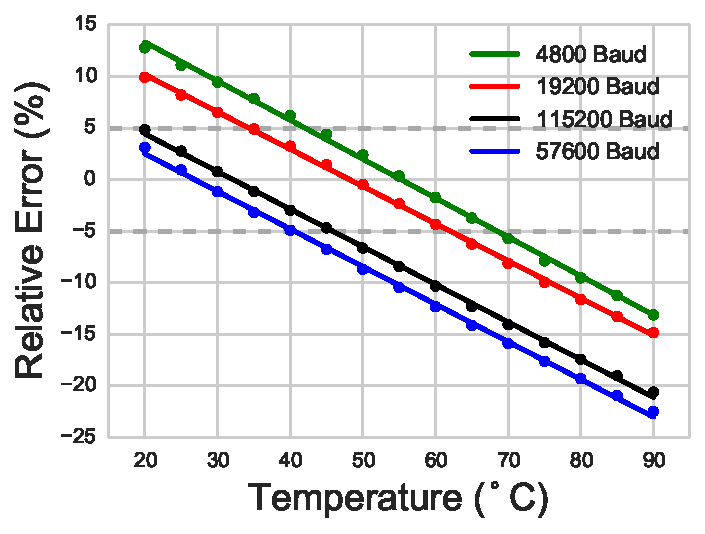
\includegraphics[width=0.475\columnwidth]{figures/baudrate_error}
    	\label{fig:baudrate_error}
    }
    \subfigure[Relative error of \acs{DCO} calibration.] {
	    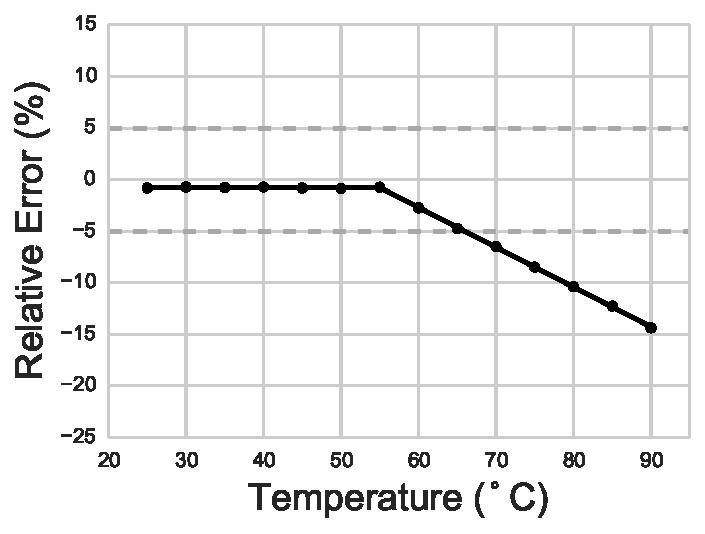
\includegraphics[width=0.475\columnwidth]{figures/reboot_dco_drift}
	    \label{fig:reboot_drift}
	}
	\subfigure[Relative error of corrected baudrate.] {
	    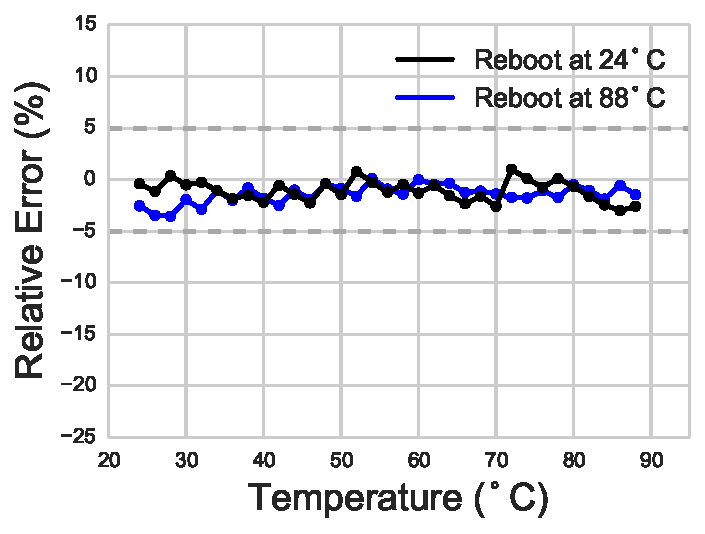
\includegraphics[width=0.475\columnwidth]{figures/baudrate_correction_error}
	    \label{fig:baudrate_look_up_error}
	}
	\subfigure[Values of baudrate correction look-up table.] {
	    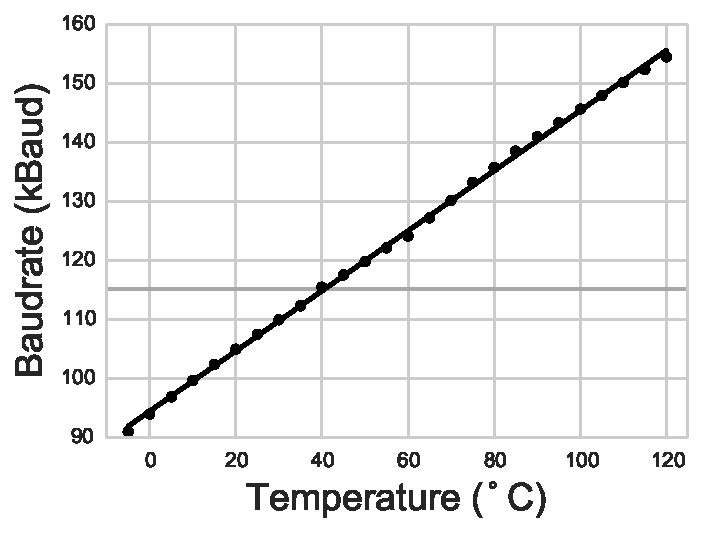
\includegraphics[width=0.475\columnwidth]{figures/baudrate_correction_table}
	    \label{fig:baudrate_look_up}
	}
	\caption{\acs{UART} and \acs{DCO} calibration errors over temperature. The dotted gray line indicates $\pm5\%$ \acs{UART} tolerance.}
\end{figure}

We then measured the relative baudrate error after rebooting over temperature.
As shown in Figure~\ref{fig:reboot_drift}, the TinyOS implementation of the \ac{DCO} calibration only works until \SI{55}{\celsius}, after which it has no corrective effect on CPU frequency, making periodic \ac{DCO} calibration during program execution ineffective.
It is possible that Contiki OS~\cite{contiki-os.org} does not experience these problems as their \ac{DCO} calibration algorithm is different from TinyOS. We did not test this, however.

To not influence the operation of the rest of the microcontroller and since understanding the \ac{DCO} calibration algorithm is not the focus of this thesis, we chose not to correct \ac{DCO} drift directly, but counteract only its effect on baudrate.
To stay within the required tolerance of $\pm5\%$ relative error, we created a fixed lookup-table of ``inverse'' correction baudrates for 115.2kBaud as shown in Figure~\ref{fig:baudrate_look_up}.

Since calculation of prescaler values at runtime is very costly (requiring floating point arithmetic in a recursive algorithm) the look-up table only contains precalculated values, which are then copied into the registers at runtime.
The on-board sensor provides temperature to the \ac{UART} module, which then selects new prescaler values from the look-up table for every \SI{5}{\celsius} temperature difference, which shows up as a sawtooth pattern in Figure~\ref{fig:baudrate_look_up_error} of the resulting relative error of the corrected baudrate.

We used this correction table without change on all of our motes and did not encounter this problem again.
This shows that even with slight differences in clock drift coefficient between different motes, this is approach is enough to solve this issue for our study.

Clock drift is not an issue for the communication between the MSP430 and the CC2420, as it is connected via the \ac{SPI}, which is a synchronous master-slave bus that provides the communication clock for its slaves, requiring no synchronisation on data symbols.


\section{Patterns in Bit Error Distributions}
\label{sec:bit_error_patterns}

We designed two experiments to investigate the results of Schmidt~\etal~\cite{Schmidt2013}.
The first experiment was used to confirm their findings and also investigate the influence of hardware layout on \ac{BER} patterns, while the second experiment investigated the influence of temperature on these patterns.

\subsection{Effects of Board Layout}
\label{subsec:effects_of_board_layout}

In all our experiments we used Tmote Sky motes, which are commercial drop-in replacements for the original Telos mote design by Polastre~\etal~\cite{Polastre2005}.
We had hardware revisions available from two manufacturers: the original design from (now defunct) MoteIV Corporation and the Maxfor MTM-CM5000MSP, which uses a slightly different schematic and board layout.
Notable differences include the \SI{3}{\volt} regulator and the physical layout of the radio circuitry.

In the experiment a pair of CM5000 and original motes transmitted to two CM5000 and two original motes.
All motes were powered by the on-board voltage regulator via the USB connector, which was also used to establish serial communications with the PC.
This redundant placement shown in Figure~\ref{fig:8mote_experiment_setup} was chosen so that the same transmission was received by both types.
Over the course of six days the four transmitters sent 563,500 messages each, totaling 2,254,000 transmitted messages at power setting 2 (below \SI{-25}{\dBm}).
Since each transmission was sent to four receivers, a total of 9,016,000 receptions should have been possible.
Of those 5,280,369 were received and 2,497,744 had at least one bit error.
The experiment was located in the large climate-controlled server room in the basement, where the temperature remained within $20$--\SI{25}{\celsius} with no other changes in the environment.

\begin{figure}[t]
	\centering
	\begin{tikzpicture}
		\newcommand\receiver[5]{%
		    \begin{scope}[xshift=#1cm,yshift=#2cm,rotate=#3]
		        \draw[fill=#4] (0,0) rectangle (1,2.1);
		     	\draw[fill=black!10] (0.33,0.1) rectangle (0.66,-0.45);
		     	\draw[snake=snake, white, segment amplitude=1.75, segment length=5, line width=1.25pt] (0.1, 1.95) -- (0.9, 1.95);
		     	\node at (0.5cm, 1.05cm) {#5};
		    \end{scope}
		}
		\newcommand\transmitter[5]{%
			\receiver{#1}{#2}{#3}{#4}{#5};
		    \begin{scope}[xshift=#1cm,yshift=#2cm,rotate=#3]
		     	\draw[snake=expanding waves, segment angle=40, segment length=7] (0.5,2) -- (0.5,3);
		    \end{scope}
		}

		% new = red, old = blue
		% new transmitter
		\transmitter{3}{7}{-65}{motered}{0};
		\transmitter{3.675}{5.5}{-65}{motered}{1};		

		% new transmitter
		\transmitter{0}{2}{-65}{moteblue}{2};
		\transmitter{0.675}{0.5}{-65}{moteblue}{3};

		\receiver{13}{0}{180}{motered}{7};
		\receiver{13}{3}{180}{moteblue}{6};
		\receiver{13}{6}{180}{motered}{5};
		\receiver{13}{9}{180}{moteblue}{4};

		% labels
		\node at (3, 7.75) {CM5000};
		\node at (0, 2.8) {Original};

		\node at (3, -1.5) {Transmitters};
		\node at (10.5, -1.5) {Receivers};
	\end{tikzpicture}
	\caption{Experiment setup with four transmitters and four receivers.}
	\label{fig:8mote_experiment_setup}
\end{figure}

The CM5000 motes required to be physically closer to the receivers at the same power setting to have similar link quality as the original motes.
This might be hinting at a difference in range between the two hardware layouts, however, our experiment was not set up to systematically investigate range.

In the initial evaluation we noted some significant differences in the quality of some links, where the co-located transmitters are sending to the same receiver.
For example, the link 3--5 is of very good quality with over 99\% \ac{PRR}, however link 2--5 shows quite the opposite with less than 1\% \ac{PRR}, even though both transmitters are located at the same distance and angle from the receiver.
This confirms the findings of Baccour~\etal~\cite{Baccour2012}, specifically that link quality is anisotropic, \ie the communication range exhibits a non-spherical pattern.
More exhibitions of this behavior can be found in the complete table of link qualifiers in the Appendix as Table~\ref{tab:8mote_link_qualities}.

Further analysis revealed the same bit and symbol error patterns as first discovered by Schmidt~\etal~\cite{Schmidt2013}, which state that within any transmitted symbol, the first three \acp{MSB} are more likely to break than the \ac{LSB} and that symbols 8--15 with the \ac{MSB} set to 1 are more likely to break than 0--7.
The normalized occurance of bit errors are plotted in Figure~\ref{fig:8mote_bit_errors}, with the first 12 bytes (96 bits) consisting of the message header with partially fixed content and the remaining 80 bytes are the constant payload, made up of two 32 byte patterns of 0x0000, 0x1111, $\ldots$ 0xFFFF, and one 16 byte pattern of 0x00, 0x11, $\ldots$ 0xFF.

\begin{figure}[t]
	\subfigure[XL] {
    	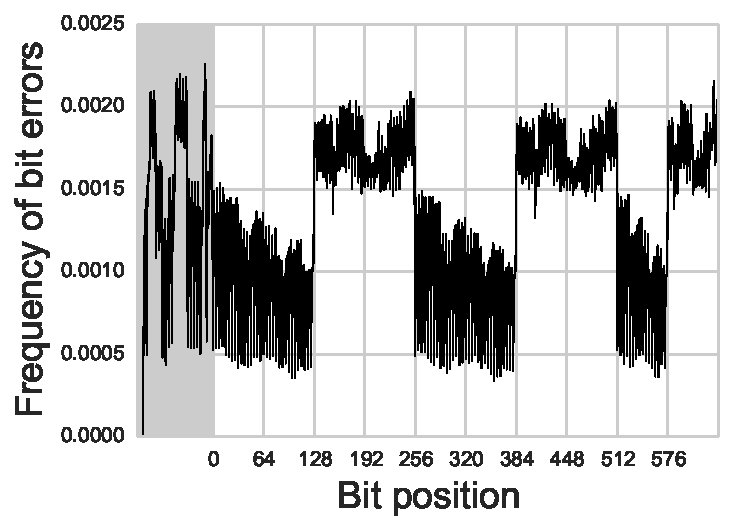
\includegraphics[width=0.475\columnwidth]{figures/8mote_0-5_xor}
    	\label{fig:8mote_bit_errors_xl}
    }
    \subfigure[L] {
	    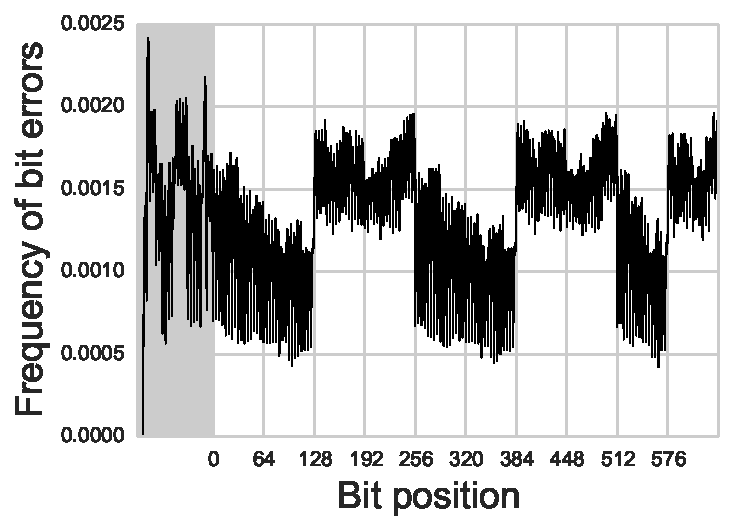
\includegraphics[width=0.475\columnwidth]{figures/8mote_1-6_xor}
	    \label{fig:8mote_bit_errors_l}
	}
	\subfigure[M] {
	    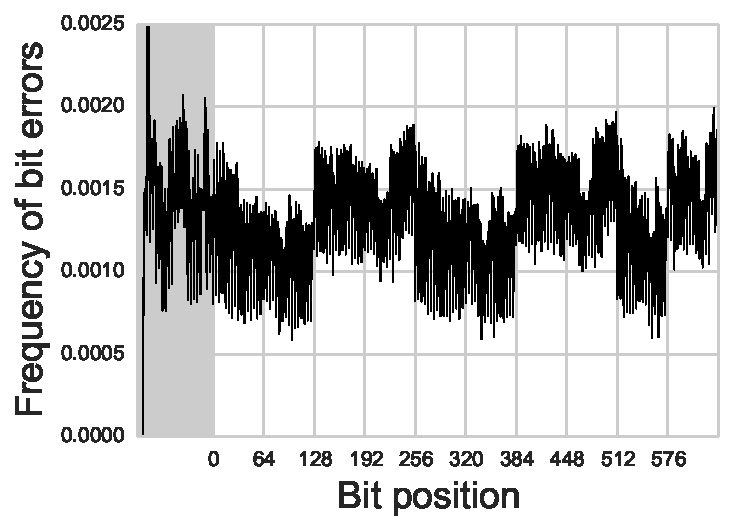
\includegraphics[width=0.475\columnwidth]{figures/8mote_2-6_xor}
	    \label{fig:8mote_bit_errors_m}
	}
	\subfigure[S] {
	    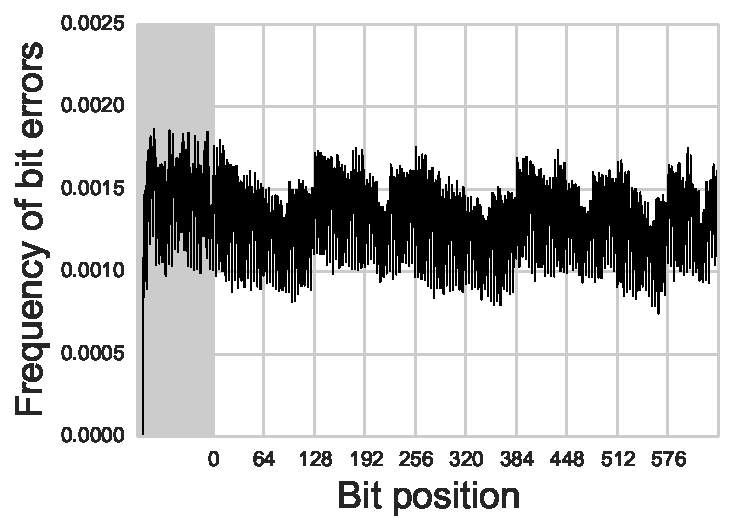
\includegraphics[width=0.475\columnwidth]{figures/8mote_2-7_xor}
	    \label{fig:8mote_bit_errors_s}
	}
	\caption{Four magnitudes of \acs{BER} patterns with fixed payload of twice 0x0000, 0x1111, $\ldots$ 0xFFFF and once 0x00, 0x11, $\ldots$ 0xFF. The message header is indicated in gray.}
	\label{fig:8mote_bit_errors}
\end{figure}

We were able to confirm the findings of Schmidt~\etal{} and extend them with a classification of the influence of symbols on \ac{BER}.
The Subfigures in \ref{fig:8mote_bit_errors} show four magnitudes of this phenomenon, ranging from an extreme to almost no difference between symbols, named XL, L, M and S.
The remaining links can be classified into these four categories as done in Table~\ref{tab:8mote_bit_error_link_classification}.
XL and L patterns seems to be more common than M and S, with 8 vs. 3 links respectively, however, the table is incomplete, since only 11 out of 16 links had enough bit errors to recognize and categorize the pattern.

Schmidt~\etal{} also looked into the burstiness of errors and showed in their research that burst errors are not independently distributed.
The authors explained the drop from 4-bit bursts to 5-bit bursts with the added difficulty of corrupting a minimum of 7 bits to overcome the minimum Hamming distance of 12 between two symbol's chip sequences.
They also hypothesized that a similar drop would occur between 8-bit and 9-bit bursts, but were unable to confirm this, due to their limited sample size.
With our larger sample size we can confirm their hypothesis, with the drop quite noticeable in Figure~\ref{fig:8mote_xl_burst}.

\begin{table}[ht]
	\begin{tabularx}{\linewidth}{|c*{4}{|c}|}
	\hline
	\T \cellcolor{slightgray} Receiver	& \multicolumn{1}{X|}{\cellcolor{motered} \centering Sender 0} & \multicolumn{1}{X|}{\cellcolor{motered} \centering Sender 1} & \multicolumn{1}{X|}{\cellcolor{moteblue} \centering Sender 2}	& \multicolumn{1}{X|}{\cellcolor{moteblue} \centering Sender 3}\\
	\hline

	\cellcolor{moteblue}\T 4 & S  & \cellcolor{slightgray} & \cellcolor{slightgray} & \cellcolor{slightgray}   \B\\
	\hline
	\cellcolor{motered}\T  5 & XL & XL & L & XL \B\\
	\hline
	\cellcolor{moteblue}\T 6 & XL & L  & M & \cellcolor{slightgray}   \B\\
	\hline
	\cellcolor{motered}\T  7 & L  & \cellcolor{slightgray} & S & L  \B\\
	\hline 
	\end{tabularx}

	\caption{Classification of all links with enough absolute bit errors (otherwise gray).}
	\label{tab:8mote_bit_error_link_classification}
\end{table}

\begin{figure}[t]
	\subfigure[XL burst error distribution.] {
    	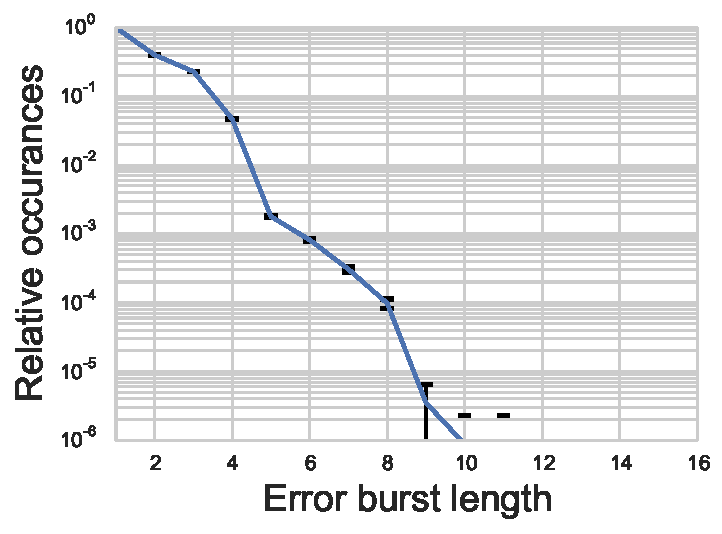
\includegraphics[width=0.475\columnwidth]{figures/8mote_0-5_burst}
    	\label{fig:8mote_xl_burst}
    }
    \subfigure[S burst error distribution.] {
	    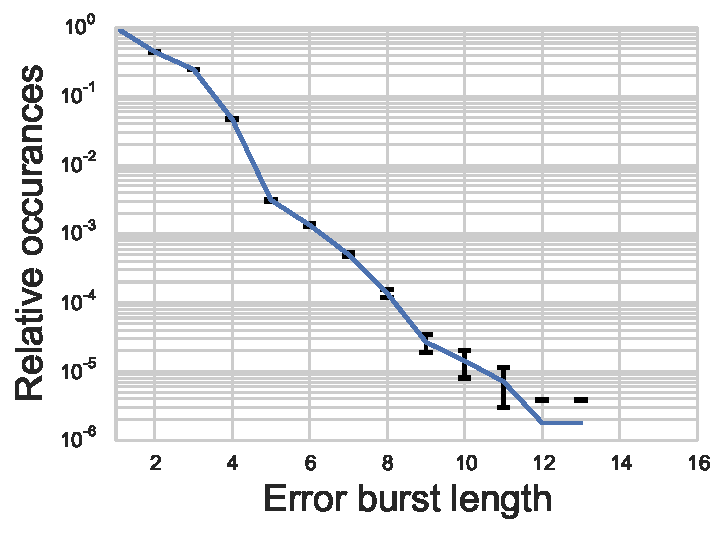
\includegraphics[width=0.475\columnwidth]{figures/8mote_2-7_burst}
	    \label{fig:8mote_s_burst}
	}
	\caption{The burst error distributions of XL and S magnitudes show more longer burst errors in S magnitude. The error bars denote 99\% confidence intervals.}
	\label{fig:8mote_burst_error}
\end{figure}

We cannot see any correlation between the four \ac{BER} pattern classifications and burst error distribution or any other variable.
We therefore believe the magnitude of these patterns to be a result of the analog circuits of the radio, something that cannot be changed or improved by software.

\subsection{Effects of Temperature}
\label{subsec:effects_of_temperature}

To investigate the influence of temperature on \ac{BER} patterns, we used the CM5000 motes in the temperature boxes as described in Section~\ref{sec:temperature_box}.
To minimize signal disturbance we mounted the boxes in the storage room on wooden posts, so that they were floating in free space.
We placed the boxes at a fixed distance of \SI{280}{\centi\metre} to each other and controlled link quality sorely by rotating the antenna.

We ran three experiments with the same constant payload as described in the Subsection~\ref{subsec:effects_of_board_layout} but with power setting 3 (\SI{-25}{\dBm}) at \SI{30}{\celsius}, \SI{50}{\celsius} and \SI{70}{\celsius}.
Due to the decrease of link quality at higher temperatures, discussed in detail in Section~\ref{sec:packet_reception_rate}, we had to adjust mote rotation to regulate \ac{BER} at these temperatures, therefore small differences in absolute bit errors are present.
However, Figure~\ref{fig:temperature_bit_errors} shows no significant difference between \ac{BER} patterns at all three temperatures and therefore we did not pursuit this further.

\begin{figure}[t]
	\subfigure[\acs{BER} pattern at \SI{50}{\celsius}.] {
    	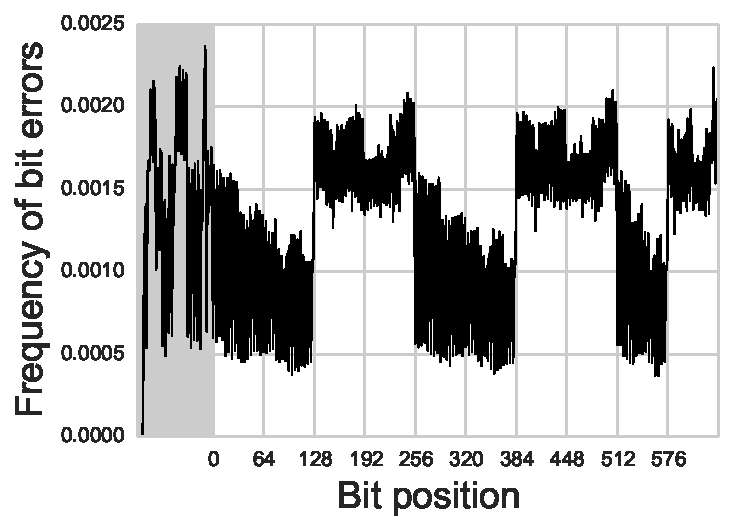
\includegraphics[width=0.475\columnwidth]{figures/temperature_1_5}
    	\label{fig:temperature_bit_errors_30}
    }
    \subfigure[\acs{BER} pattern at \SI{70}{\celsius}.] {
	    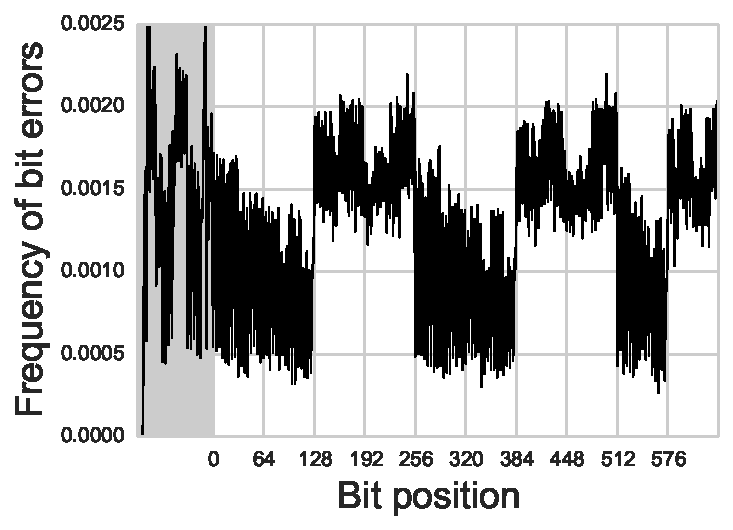
\includegraphics[width=0.475\columnwidth]{figures/temperature_0_6}
	    \label{fig:temperature_bit_errors_70}
	}
	\caption{\acl{BER} patterns show no difference between \SI{30}{\celsius}, \SI{50}{\celsius} and \SI{70}{\celsius}. The pattern at \SI{30}{\celsius} is omitted, since it is redundant.}
	\label{fig:temperature_bit_errors}
\end{figure}


\subsection{Pattern Anomalies}
\label{subsec:pattern_anomalies}

Even though the vast majority of experiment evaluations confirmed these patterns, there were two runs with  drastically different outcome.
We were very surprised to find a second, completely opposite \ac{BER} pattern as shown in Figure~\ref{fig:anomalie_bit_error}.
Here the symbols 0-7 show a higher average \ac{BER} and a less pronounced 4-bit saw-tooth pattern than symbols 8-15.
The pattern almost looks like an ``inverse'' of those described earlier.

The first time it occurred, we attributed this to influences of the environment and discarded it.
Two months later, this pattern occurred again with different hardware in a different setup in a different environment.
Both times, the motes were exposed to high temperature (>\SI{70}{\celsius}) over several hours, however, we were unable to confirm if this indeed triggered the pattern.
This pattern remained for days, regardless of temperature, link quality or message payload.

We cannot envision a source of interference capable of fundamentally changing this \ac{BER} distribution and neither does a permanent change of the radio chip's hardware at high temperature seem possible.
The CC2420 radio is rated to be operated at temperatures up to \SI{85}{\celsius} and to be stored at up to \SI{150}{\celsius}, while our experiments where limited to at most \SI{90}{\celsius} for a few hours.

Since we could not find any other reference to this pattern in literature and due to the rarity of this occurrence in our experiments and the difficulty of its repeatability, we decided to focus on investigating the ``normal'' patterns.

\begin{figure}[t]
	\subfigure[First occurance.] {
    	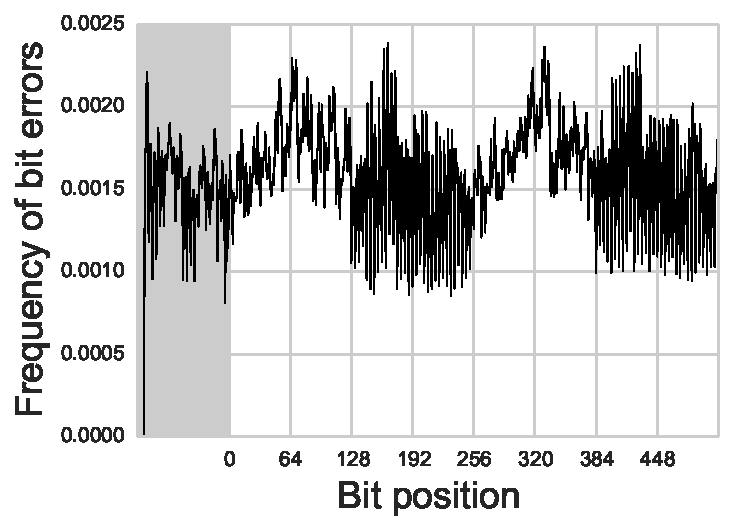
\includegraphics[width=0.475\columnwidth]{figures/anomaly_first}
    	\label{fig:anomalie_earlier}
    }
    \subfigure[Second occurance.] {
	    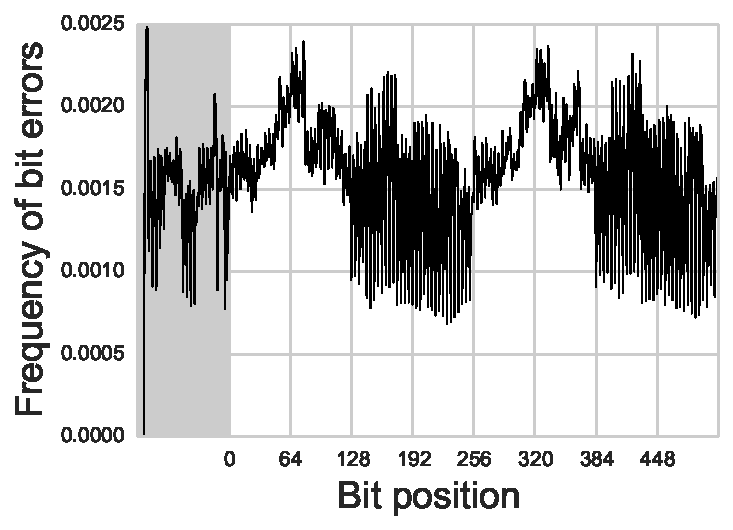
\includegraphics[width=0.475\columnwidth]{figures/anomaly_second}
	    \label{fig:anomalie_later}
	}
	\caption{``Inverted'' \acs{BER} pattern anomaly of constant data. Only the first two 32 byte patterns are shown.}
	\label{fig:anomalie_bit_error}
\end{figure}




\section{Packet Reception Rate}
\label{sec:packet_reception_rate}

The effect of temperature and other environmental factors on link quality has most thoroughly been investigated with the conclusion that all measurements of link quality deteriorate with higher temperature, as one would expect~\cite{Wennerstrom2013, Boano2013, Boano2014, Zuniga2013}.
However, Boano~\etal{} showed in their experiments that this behavior is not symmetrical, since heating the transmitter caused a more significant drop in \ac{PRR} than heating the receiver~\cite{Boano2013}.

In this experiment we used the same physical setup as described in Section~\ref{subsec:effects_of_temperature}, but with random payload as message content.
We fixed mote rotation to create a link that is just starting to deteriorate at \SI{50}{\celsius}, so that at low temperatures the link is of good quality, while at very high temperatures the link will experience high \ac{BER}s.

We increased the temperature of the mote in box 0 in steps of \SI{5}{\celsius} and \SI{10}{\celsius} up to \SI{80}{\celsius} and kept the mote on box 1 at constant \SI{30}{\celsius}, while sending 180.000 messages back and forth.
Then we repeated this, but heated box 1 and kept box 0 temperature constant.
To cancel out environmental factors we ran this experiment four times over two days, so we could then pick the two results with the least interference.

For the evaluation we plotted the normalized \ac{PRR} of messages sent from one mote and received by the other mote over temperature and time and included \ac{BER} and \ac{LQI} and \ac{RSSI} values to illustrate link quality.
Figure~\ref{fig:prr_link_01} shows messages sent from mote 0 addressed to mote 1 for both temperature cycles, while Figure~\ref{fig:prr_link_10} shows the opposite direction.
It becomes immediately clear that a higher temperature of either transmitter or receiver makes the link quality worse, validating the findings of Boano~\etal{} and Wennerstr{\"o}m~\etal~\cite{Boano2013, Wennerstrom2013}.
However, this relationship is neither linear nor symmetrical.


\subsection{Effects of Temperature on \acs{PRR} and \acs{BER}}

In Figure~\ref{fig:prr_link_01} the decrease in \ac{PRR} is small and relatively symmetrical up to about \SI{65}{\celsius}, however, past that point we see a dramatic change, with the increments in temperature translating very strongly into significant drops in \ac{PRR}.
The drop in \ac{PRR} is not symmetrical and becomes much more pronounced, when the receiver is heated than when the transmitter is heated, especially visible in the last increment from \SI{70}{\celsius} to \SI{80}{\celsius}.

This asymmetry is even more extreme in link 1-0, shown in Figure~\ref{fig:prr_link_10}, where heating the receiver beyond \SI{70}{\celsius} will cause an almost complete loss of message reception.
Interesting is the little dip in \ac{PRR} around \SI{50}{\celsius} in Figure~\ref{fig:prr_link_10_receiver}, which was present in this link in all four experiments with varying intensity. We suspect that this is a non-linearity in the radio, cases of which have also been reported by Boano~\etal

The \ac{BER} acts like an inverse function of \ac{PRR}, since higher \ac{BER} yields more messages with at least one bit error.
Noise on \ac{PRR} is visible in the standard deviation of \ac{BER} as exemplified by Figure~\ref{fig:prr_link_10_transmitter}.


\subsection{Effects of Temperature on \acs{LQI} and \acs{RSSI}}

The \ac{LQI} is a very good mirror of the \ac{PRR} of messages without error.
When the receiver is kept at a constant temperature, the values decrease almost linearly with temperature of the transmitter.
This is not the case when the receiver is heated, where a linear correlation to temperature , but is still very similar to the behavior of \ac{PRR}.
We therefore can confirm that \ac{LQI} is a good source for an estimate on \ac{PRR}.

This is very much not the case with \ac{RSSI}, which has much lower resolution that \ac{LQI} and exhibits hysteresis and non-linearities~\cite{Boano2013}.
While in Figure~\ref{fig:prr_link_01}, \ac{RSSI} ends up being lower when the receiver is heated than when it is constant, Figure~\ref{fig:prr_link_10} shows very similar values, even though \ac{PRR} is radically different.

It is also noteworthy that contrary to \ac{LQI}, \ac{RSSI} attempts to describe signal strength (\ie the power level being received by the antenna), which of course does not change, when the transmitter is at constant temperature.
Therefore, without temperature information, the \ac{RSSI} value is misleading, since it represents the power level not at the antenna, but at the signal amplifying stage of the radio. 
Therefore \ac{RSSI} is usable for a very inaccurate estimate of link quality at best, with little to no difference between receiver and transmitter temperature.


\subsection{Discussion}

Our data strongly implicates the receiver as being more vulnerable than the transmitter to an increase in temperature, especially above \SI{65}{\celsius}.
These results are very much incompatible with the findings of Boano~\etal~\cite{Boano2013}, which is surprising since the only two differences between our experiment and theirs is the temperature range and the additional usage of the CC2520~\cite{cc2520} radio, which is very similar to the CC2420~\cite{cc2420}.
However, these differences should not account for completely opposing results.

Research by Bannister~\etal~\cite{Bannister2008} saw an asymmetry in output and received input power when heating transmitter and receiver separately.
At the same time, they measured \ac{PER} and found that above \SI{-90}{\dBm} \ac{RSSI}, temperature had little to no influence, while below that \ac{RSSI} value, \ac{PER} increased.
The authors concluded that the CC2420 \acl{LNA} stage is less efficient at high temperature, which would manifest itself in a significant increase in \ac{PER} (or a \emph{decrease} in error-free \ac{PRR}) on the receiver.
However, the \ac{RSSI} behavior in Figure~\ref{fig:prr_link_10} does not reflect a general truth of the results by Bannister~\etal{} and furthermore suggests no direct correlation between \ac{RSSI} and \ac{PRR}.

We noticed a strong focus in such research on understanding the impact of temperature on output and input signal power, however, it seems that \ac{RSSI} does not actually correspond to link quality in general.
From our data, a combination of \ac{LQI} and temperature seems to have the best correlation to \ac{PRR}, therefore we want to examine how we can use temperature to improve \ac{PRR} in these conditions.

\begin{figure}[t]
	\subfigure[Constant receiver, increasing \newline transmitter temperature.] {
		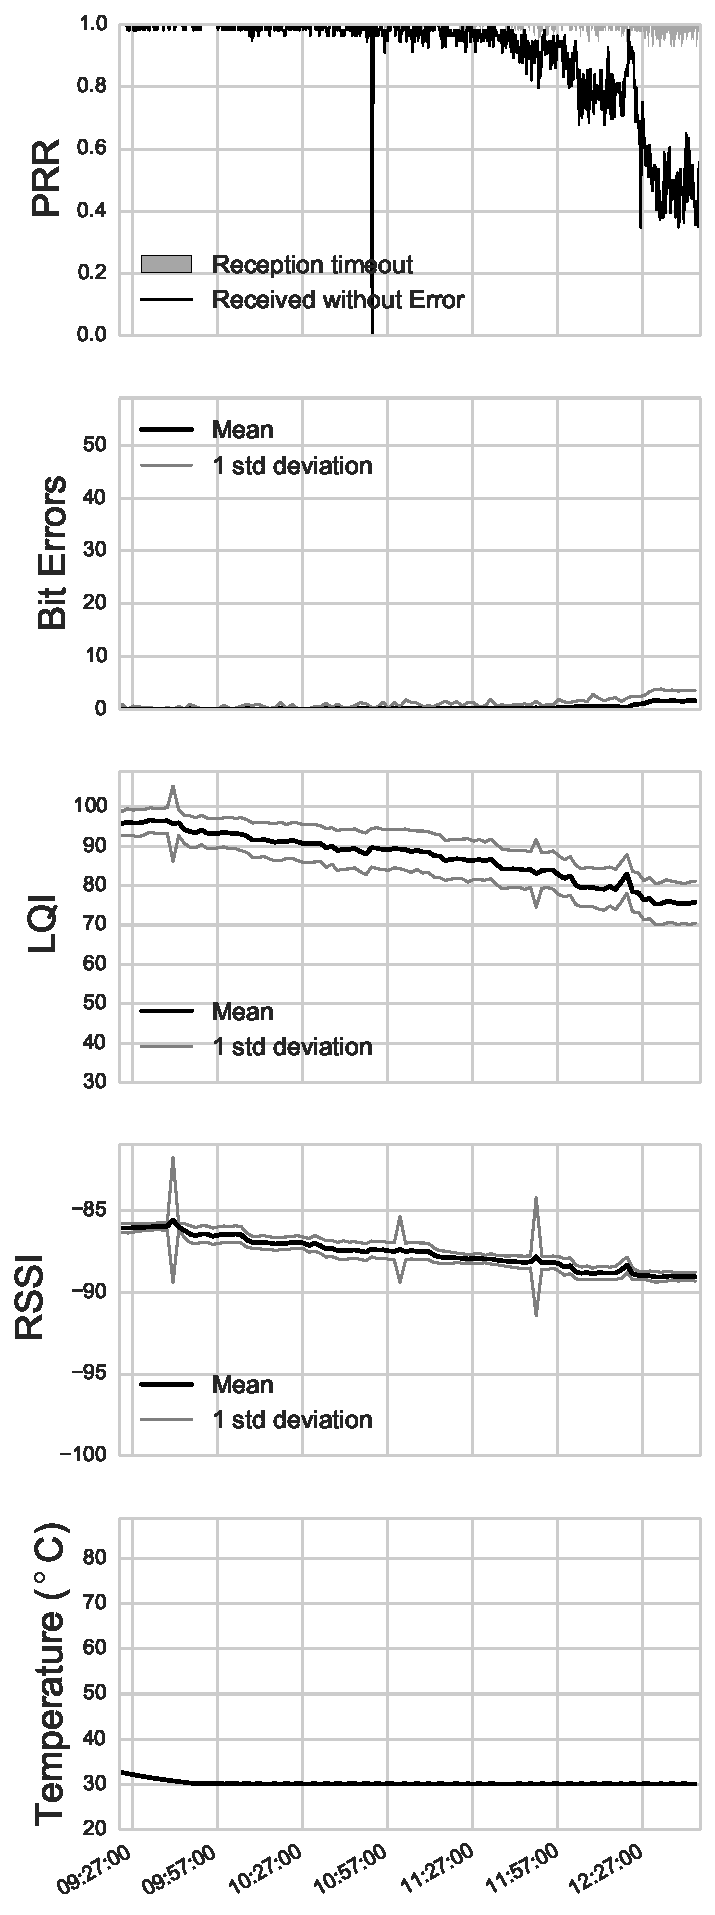
\includegraphics[width=0.475\columnwidth]{figures/prr_0-1_transmitter}
		\label{fig:prr_link_01_transmitter}
	}
	\subfigure[Increasing receiver, constant \newline transmitter temperature.] {
		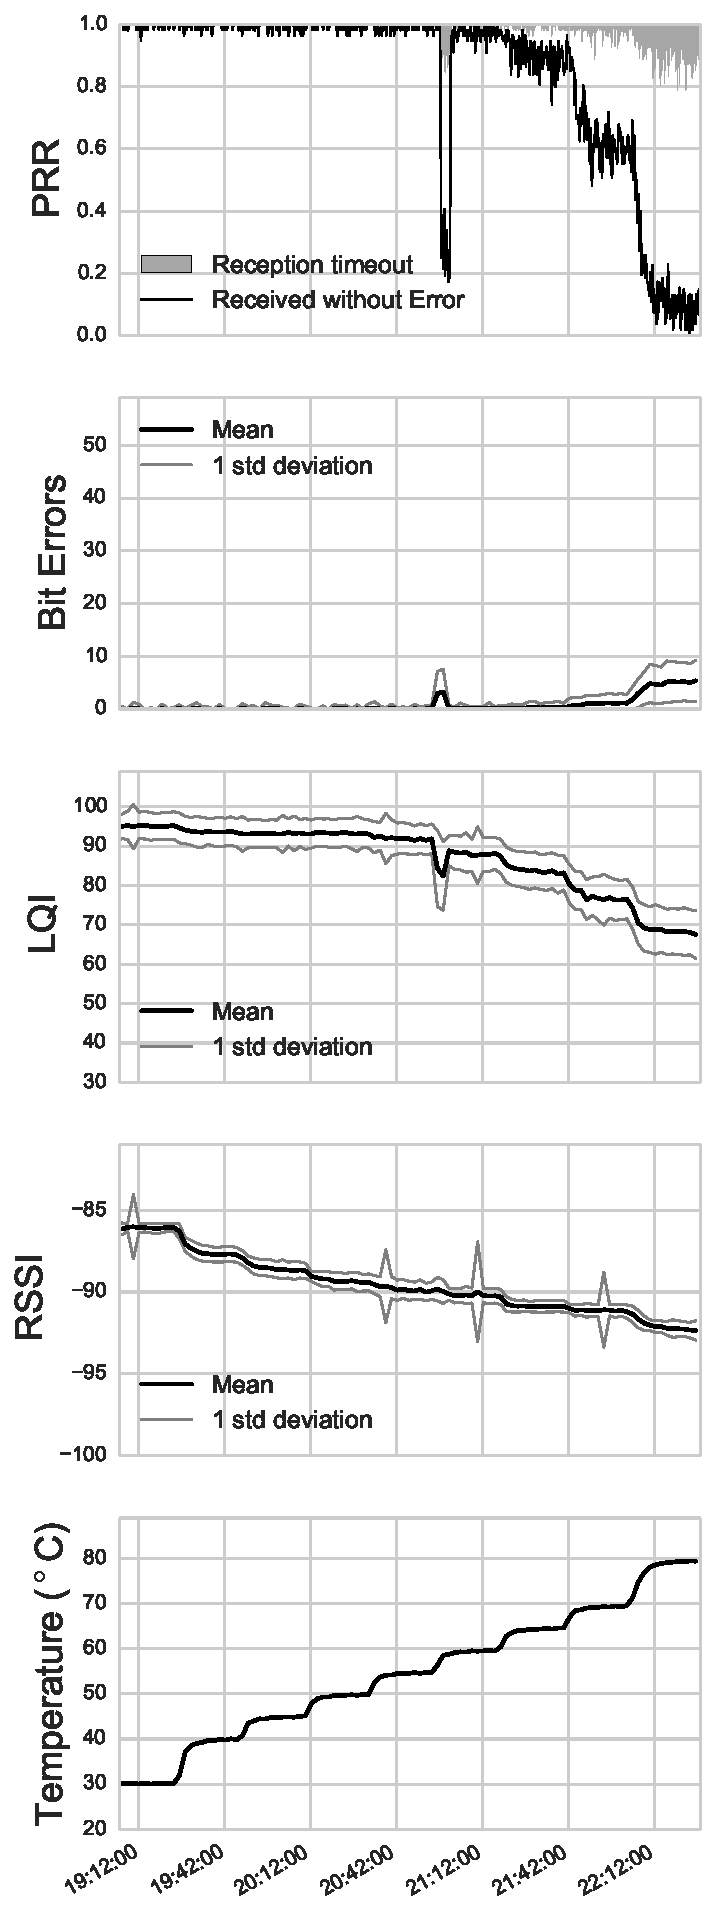
\includegraphics[width=0.475\columnwidth]{figures/prr_0-1_receiver}
		\label{fig:prr_link_01_receiver}
	}
	\caption{\acs{PRR} and link quality of messages received by mote \textbf{1} vs. temperature. For transmitter temperature see Figure~\ref{fig:prr_link_10}.}
	\label{fig:prr_link_01}
\end{figure}

\begin{figure}[t]
	\subfigure[Increasing receiver, constant \newline transmitter temperature.] {
		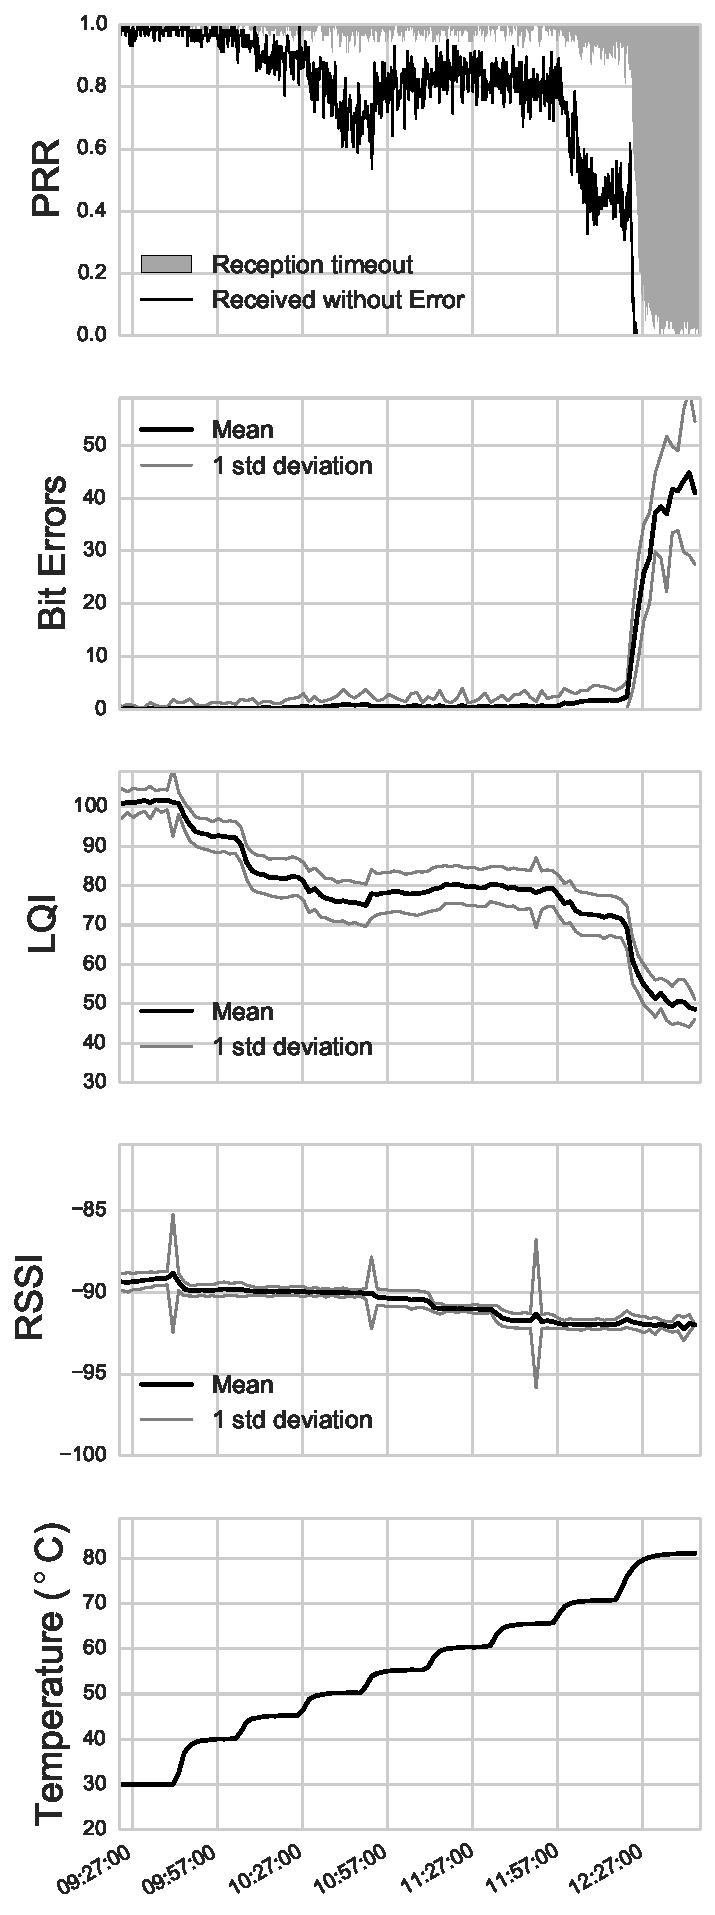
\includegraphics[width=0.475\columnwidth]{figures/prr_1-0_receiver}
		\label{fig:prr_link_10_receiver}
	}
	\subfigure[Constant receiver, increasing \newline transmitter temperature.] {
		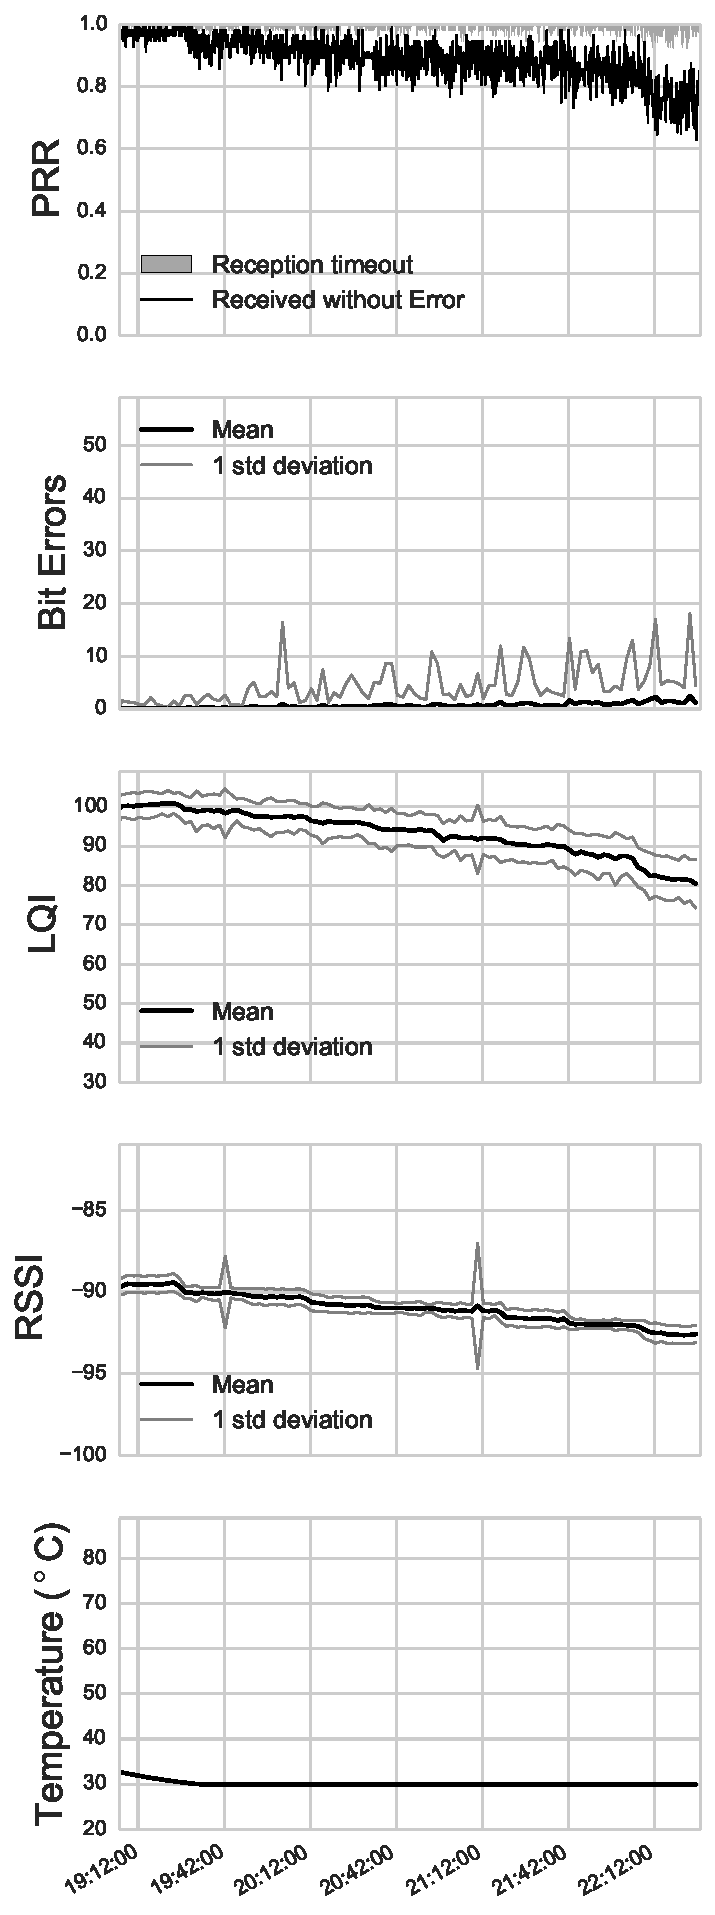
\includegraphics[width=0.475\columnwidth]{figures/prr_1-0_transmitter}
		\label{fig:prr_link_10_transmitter}
	}
	\caption{\acs{PRR} and link quality of messages received by mote \textbf{0} vs. temperature.  For transmitter temperature see Figure~\ref{fig:prr_link_01}. The asymmetry in \acs{PRR} shows much more clearly here.}
	\label{fig:prr_link_10}
\end{figure}


